%!TEX root = ../../Master.tex

\section{Mapping a Multistory Building Complex}

In this section the method on how to represent a floor and what problems that ties to mapping a complex will be described.

\subsection{Representing a Floor}

Every decision and every change direct is a vertex in our graph, is modelled by vertices connected with edges. \label{e_vertex} Any vertex that connects a floor with another, is called an exit vertex, and can be classified as stairs, elevators or 'others', which could be ground floor entrances or second floor walkways. Vertices that does not classify as one of the previously mentioned are doors, intersection and other positions where a change of direction can occur. Connecting the vertices are edges with a weight, which could be weighted with the distance in meters from one vertex to another. Figure \ref{fig:floorplan_graf} illustrates how the graph will look like on a floor plan for a existing building. The circles are vertices and lines are edges.

\subsection{Representing Floor Relations in a Building Complex}

When mapping a building complex, a problem arises when trying to define the floor on which the user is situated. Since 'the second floor' could be in any two story building, there needs to be a way of differentiating between buildings. There is however, a better way of storing this information in a different way, than just adding a building ID tag to each vertex. Instead, the system will mark all floors individually, disregarding their real world relations.

If a building with three floors and one with two floors are to be represented, the floors will be numbered 1 through 5. The building with the three floors could have its first floor numbered 1, second numbered 2 and third numbered 3. The building with two floors would then have its first floor numbered 4 and second floor numbered 5. When modelled, the floors will be sorted by their vertex id's and sorted sequential as seen on the figure. This means that the second floor in two separate buildings will not have the same floor id. The thick straight line between 3 and 4, indicates a separation between two buildings, but is only present in this illustration and only indirectly included in the implementation. As seen on the figure, there is an exit vertex(a) at floor 1 connected to an exit vertex at floor 2, which could represent a stairway or an elevator. The connection(c) between 1 and 4 is possible as both of these floors is at ground level. There is also a connection(b) between 2 and 5 even though the floors are not at ground level or in the same building. This could be a representation of a walkway connecting them.

\subsection{Implication of graph directions}

When mapping a building, the choice of using a directed graph or not, has to be considered. Most hospitals will not require a directed graph, since the building will have a high level of accessibility. But if the solution were to be used in a building with a one directional path, such as an escalator, a directed graph would be required in order to avoid leading people against the direction. Creating a directed graph is not a complicated process, but it does entail some restrictions when evaluating the routes. A system that does not expect to encounter a directed graph, could reduce some calculation by assuming that the path from any given vertex A to any given vertex B would be the same from B to A. Another issue that is not addressed in this solution, is the difference between travelling up and down a staircase. This could also be handled through the use of a directed graph.


\begin{figure}[ht!]
    \centering
    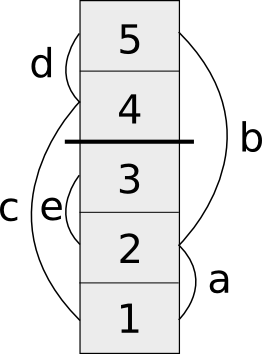
\includegraphics[width=0.5\textwidth]{PekhoeS}
    \caption{Visual representation of floors}n
    \label{fig:PekhoeS}
  \end{figure}

\begin{figure}[ht!]
    \centering
    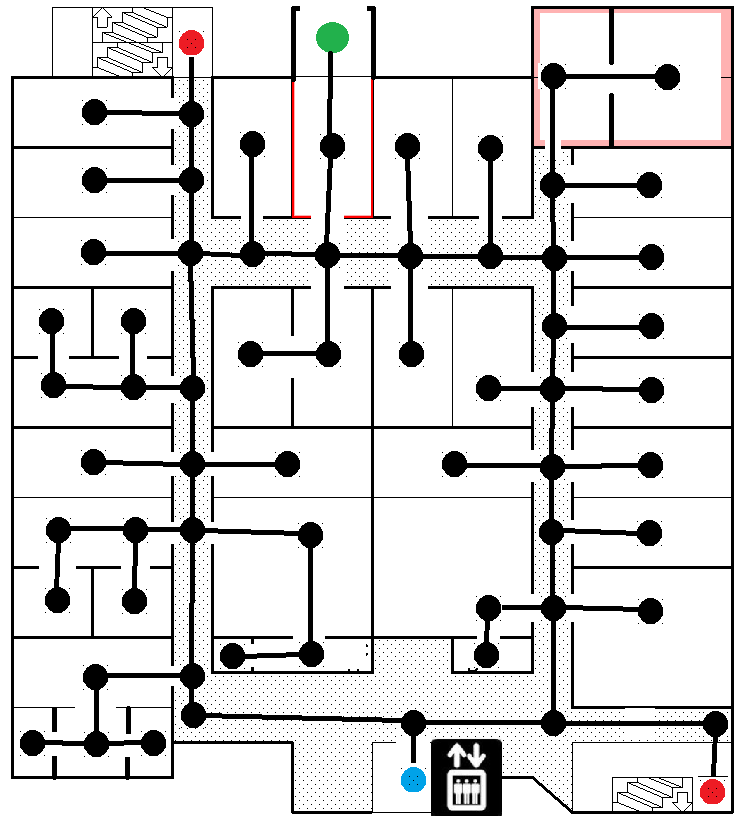
\includegraphics[width=0.5\textwidth]{floorplan_graf}
    \caption{representation of a graph on a floor plan.}
    \label{fig:floorplan_graf}
  \end{figure}

